%\documentclass[journal]{IEEEtran}
\documentclass[12pt, draftcls, onecolumn]{IEEEtran}
\makeatletter
% journal (default) and conference
\def\subsubsection{\@startsection{subsubsection}% name
                                 {3}% level
                                 {\z@}% indent (formerly \parindent)
                                 {0ex plus 0.1ex minus 0.1ex}% before skip
                                 {0ex}% after skip
                                 {\normalfont\normalsize\bfseries}}% style
\makeatother
\usepackage[T1]{fontenc}% optional T1 font encoding
%\usepackage{graphicx}
\usepackage{subfigure}
\usepackage{ulem}
\usepackage{tabu}
\usepackage{amsmath}
\DeclareMathOperator*{\argmax}{arg\,max}
\allowdisplaybreaks
\usepackage{hhline}
\usepackage{yfonts,color}
\usepackage{soul,xcolor}
\usepackage[options]{algorithm2e}
\usepackage{algorithm}
\usepackage{verbatim}
\usepackage{amsmath}
\allowdisplaybreaks
\usepackage{amssymb}
\usepackage{amsthm}
\usepackage{float}
\usepackage{bm}
\usepackage{url}
\usepackage{array}
\usepackage{cite}
\usepackage{graphicx}
\usepackage{framed} % for frame
\usepackage{balance} % balance
\usepackage{epsfig,epstopdf}
\usepackage{booktabs}
\usepackage{courier}
\usepackage{subfigure}
\usepackage{enumerate}
\usepackage[export]{adjustbox}
\newtheorem{definition}{Definition}
\newtheorem{theorem}{Theorem}
\newtheorem{lemma}[theorem]{Lemma}
\newtheorem{proposition}[theorem]{Proposition}
%\newtheorem{proposition}{Proposition}
\newtheorem{corollary}[theorem]{Corollary}
\newtheorem{assumption}{Assumption}
\newtheorem{remark}{Remark}
\newcommand{\rom}[1]{\uppercase\expandafter{\romannumeral #1\relax}}
\usepackage{color}
\usepackage{soul,xcolor}
\newcommand{\nm}[1]{{\color{blue}\text{\bf{[NM: #1]}}}}
\newcommand{\sst}[1]{\st{#1}}
\newcommand{\gs}[1]{{\color{orange}\bf{[GS: #1]}}}
\newcommand{\remove}[1]{{\color{magenta}{\bf REMOVE: [#1]}}}
%\newcommand{\nm}[1]{}
%\newcommand{\sst}[1]{}
%\newcommand{\gs}[1]{}
%\newcommand{\remove}[1]{}
\newcommand{\add}[1]{{\color{red}{#1}}}
\newcommand{\ull}[1]{\textbf{\color{red}\ul{#1}}}
%\pagestyle{empty}
\normalem
\begin{document} 
\setulcolor{red}
\setul{red}{2pt}
\title{ECE64700: Homework IV}
\author{Bharath Keshavamurthy}
\maketitle
\section{Markov Decision Processes - An Energy Harvesting Radio Node}
\subsection{System Model}
We consider a single energy harvesting radio node with an MDP agent running as a part of its decision engine solving for the optimal transmission policy considering channel fading states and battery energy levels.
\\The channel fading states $g_k$ realize from the following set i.i.d over time with a uniform probability distribution $\mathbb{P}(g_k\ =\ \gamma_i)\ =\ \theta_i\ =\ \frac{1}{N}$.
\begin{equation}\label{1}
    \mathcal{G}\ \equiv\ \{\gamma_i,\ i\ =\ 1,\ 2,\ 3,\ ...,\ N\}
\end{equation}
The battery states $Q_k$ realize from the following set.
\begin{equation}\label{2}
    \mathcal{Q}\ \equiv\ \{m E_0,\ m\ =\ 0,\ 1,\ 2,\ 3,\ ...,\ M\}
\end{equation}
The battery state update procedure is as follows.
\begin{equation*}
    Q_{k+1}\ =\ \min\{Q_k - w_k + a_k,\ M E_0\}
\end{equation*}
where,
\\$w_k \in \{0,\ E_0\}$ is the amount of energy spent by the radio node during transmission, and
\\$a_k \in \{0,\ E_0\}$ is modelled as a Bernoulli i.i.d process with $\mathbb{P}(a_k\ =\ E_0)\ =\ p$ as the success probability and $\mathbb{P}(a_k\ =\ 0)\ =\ (1-p)$ as the failure probability.
\subsubsection{The State Space} The state space for the MDP agent is denoted by $\mathcal{S}$.
\\In time-slot $k$, we represent the state of the process as a 2-tuple or a pair $(Q_k,\ g_k)$ where,
\\$Q_k \in \mathcal{Q}$ is defined as the current battery level or the amount of energy available in the battery in time-slot $k$, and
\\$g_k\ \in \mathcal{G}$ is defined as the current state of the fading channel.
\\The dimensionality of the state space is given by $|\mathcal{S}|\ =\ MN\ =\ 110$ possible states.
\\Therefore, concretely,
\begin{equation}\label{3}
    \mathcal{S}\ \equiv\ \{(Q_k,\ g_k)\ |\ Q_k \in \mathcal{Q},\ g_k\ \in \mathcal{G}\}
\end{equation}
\subsubsection{The Action Space} The action space of the MDP agent is denoted by $\mathcal{U}$.
\\In time-slot $k$, the actions available to the MDP agent are,
\begin{equation}\label{4}
    u_k\ =\ 
    \begin{cases}
    0,\ \text{if $Q_k\ =\ 0$ and $g_k \in \mathcal{G}$}\\
    \{1,\ 2,\ 3,\ ...,\ i\},\ \text{if $Q_k\ \not=\ 0$ and $g_k\ =\ \gamma_i \in \mathcal{G}$}
    \end{cases}
\end{equation}
If the battery is dead, the radio node cannot transmit anything. Hence, the only available action in states with $Q_k\ =\ 0$ is to remain idle, i.e. $u_k\ =\ 0$.
\\If there are units of energy in the battery (the units are discretized in steps of $E_0$ as it is evident from equation (\ref{2})), the actions of the radio node depends on the realization of the fading state of the channel.
\subsubsection{The Transition Model}
The transition model of the process if given by,
\begin{equation}\label{5}
    (Q_{k+1},\ g_{k+1})\ =\ 
    \begin{cases}
        (Q_k,\ g_{k+1}),\ \text{if $u_k\ =\ 0$ and $a_k\ =\ 0$ \textbf{with probability $\frac{1-p}{N}$}}\\
        (Q_k - E_0,\ g_{k+1}),\ \text{if $u_k \not= 0$ and $a_k\ =\ 0$ \textbf{with probability $\frac{1-p}{N}$}}\\
        (\min\{Q_k + E_0,\ M E_0\},\ g_{k+1}),\ \text{if $u_k\ =\ 0$ and $a_k\ =\ E_0$ \textbf{with probability $\frac{p}{N}$}}\\
        (Q_k,\ g_{k+1}),\ \text{if $u_k\ \not= 0$ and $a_k\ =\ E_0$ \textbf{with probability $\frac{p}{N}$}}
    \end{cases}
\end{equation}
\subsubsection{The Reward Metric}
The reward metric is denoted by $r_k\ =\ R(s_k,\ u_k)$.
\\In time-slot $k$, we model the reward to the MDP agent as the number of bits it could transmit over the channel given the process state $s_k\ =\ (Q_k,\ g_k) \in \mathcal{S}$, i.e. $r_k\ =\ u_k$.
\subsection{The Problem Formulation}
In order to solve for the optimal policy to be followed by the MDP agent residing in the decision engine of the energy harvesting radio node, we formulate the following problem which turns out to be the \textbf{Bellman Optimality Equation for Infinite Horizon Discounted Reward Problems}.
\begin{equation}\label{6}
    V^*(s)\ =\ \max_{u \in \mathcal{U}(s)}\ R(s,\ u) + \rho \sum_{s' \in \mathcal{S}}\ P_{s'|s,u}V^*(s')
\end{equation}
where,
\\$\rho\ =\ 0.9$ is the discount factor,
\\$P_{s'|s,u}$ is the transition probability detailed in the transition model (\ref{5}), and
\\$R(s,\ u)$ is the reward received in state $s$ after taking action $u$.
\subsection{Solution Methodology and Performance}
\subsubsection{The Algorithms}
We employ the Value Iteration Algorithm and the Policy Iteration Algorithm to solve for the optimal policy as shown below.
\begin{itemize}
    \item \textbf{Value Iteration}
    \begin{algorithm}[H]
        \SetAlgoLined
        \KwResult{The optimal policy $\mu^*$ and optimal value function $V^*(s), \forall s \in \mathcal{S}$}
         \textbf{Initialization}: Start with an initialization of the value function, $V_0(s)\ =\ 10^{-5},\ \forall s \in \mathcal{S}$;
         \\\While{$\forall s \in \mathcal{S}, V_{k+1}(s) \not= V_{k}(s)$}{
          $V_{k+1}(s)\ =\ \max_{u \in \mathcal{U}(s)}\ \Big[u + \rho \sum_{s' \in \mathcal{S}}\ P_{s'|s,u}V_{k}(s')\Big]$\\
          $u_k(s)\ =\ \argmax_{u \in \mathcal{U}(s)}\ \Big[u + \rho \sum_{s' \in \mathcal{S}}\ P_{s'|s,u}V_{k}(s')\Big]$
         }
         Return $V^*(s),\ \forall s \in \mathcal{S}$ and $\mu^*\ =\ \{u^*(s)\ |\ s \in \mathcal{S}\}$ after convergence
        \caption{The Value Iteration Algorithm for the given MDP agent}
    \end{algorithm}
    \item \textbf{Policy Iteration}
    \begin{algorithm}[H]
        \SetAlgoLined
        \KwResult{The optimal policy $\mu^*$ and optimal value function $V^*(s), \forall s \in \mathcal{S}$}
         \textbf{Initialization}: Start with an arbitrary policy $\mu_0\ =\ \{0\ (idle),\ \forall s \in \mathcal{S}\}$ and an initialization of the value function, $V_0(s)\ =\ 10^{-5},\ \forall s \in \mathcal{S}$;
         \\\While{$\forall s \in \mathcal{S}, \mu_{k+1}(s) \not= \mu_{k}(s)$}{
          \textbf{Policy Evaluation}:
          \\$V_{\mu_k}(s)\ =\ \Big[\mu_k(s) + \rho \sum_{s' \in \mathcal{S}}\ P_{s'|s,u}V_{\mu_k}(s')\Big]$\\
          \textbf{Policy Improvement}:
          \\$\mu_{k+1}(s)\ =\ \argmax_{u \in \mathcal{U}(s)}\ \Big[u + \rho \sum_{s' \in \mathcal{S}}\ P_{s'|s,u}V_{\mu_{k}}(s')\Big]$
         }
         Return $V^*(s),\ \forall s \in \mathcal{S}$ and $\mu^*$ after convergence
        \caption{The Policy Iteration Algorithm for the given MDP agent}
    \end{algorithm}
\end{itemize}
Please refer to the provided source code (\textit{EnergyHarvestingNode.py}) for more details.
\clearpage
\subsubsection{Results of the Algorithms}
\begin{itemize}
    \item \textbf{Value Iteration}
        \\The optimal policy from the Value Iteration Algorithm is given below.\newline
        \begingroup
            \fontsize{10pt}{10pt}\selectfont
            {`0\_1': 0, `0\_2': 0, `0\_3': 0, `0\_4': 0, `0\_5': 0, `0\_6': 0, `0\_7': 0, `0\_8': 0, `0\_9': 0, `0\_10': 0,\\ `1\_1': 0, `1\_2': 0, `1\_3': 0, `1\_4': 0, `1\_5': 0, `1\_6': 0, `1\_7': 7, `1\_8': 8, `1\_9': 9, `1\_10': 10,\\ `2\_1': 0, `2\_2': 0, `2\_3': 0, `2\_4': 0, `2\_5': 5, `2\_6': 6, `2\_7': 7, `2\_8': 8, `2\_9': 9, `2\_10': 10,\\ `3\_1': 0, `3\_2': 0, `3\_3': 0, `3\_4': 0, `3\_5': 5, `3\_6': 6, `3\_7': 7, `3\_8': 8, `3\_9': 9, `3\_10': 10,\\ `4\_1': 0, `4\_2': 0, `4\_3': 0, `4\_4': 4, `4\_5': 5, `4\_6': 6, `4\_7': 7, `4\_8': 8, `4\_9': 9, `4\_10': 10,\\ `5\_1': 0, `5\_2': 0, `5\_3': 3, `5\_4': 4, `5\_5': 5, `5\_6': 6, `5\_7': 7, `5\_8': 8, `5\_9': 9, `5\_10': 10,\\ `6\_1': 0, `6\_2': 0, `6\_3': 3, `6\_4': 4, `6\_5': 5, `6\_6': 6, `6\_7': 7, `6\_8': 8, `6\_9': 9, `6\_10': 10,\\ `7\_1': 0, `7\_2': 0, `7\_3': 3, `7\_4': 4, `7\_5': 5, `7\_6': 6, `7\_7': 7, `7\_8': 8, `7\_9': 9, `7\_10': 10,\\ `8\_1': 0, `8\_2': 2, `8\_3': 3, `8\_4': 4, `8\_5': 5, `8\_6': 6, `8\_7': 7, `8\_8': 8, `8\_9': 9, `8\_10': 10,\\ `9\_1': 0, `9\_2': 2, `9\_3': 3, `9\_4': 4, `9\_5': 5, `9\_6': 6, `9\_7': 7, `9\_8': 8, `9\_9': 9, `9\_10': 10,\\ `10\_1': 1, `10\_2': 2, `10\_3': 3, `10\_4': 4, `10\_5': 5, `10\_6': 6, `10\_7': 7, `10\_8': 8, `10\_9': 9, `10\_10': 10}
        \endgroup
        \\Here, $0\_1: 0$ refers to the optimal action of remaining idle, i.e. $u_k=0$, if the process state is $(Q_k=0,\ g_k=\gamma_1)$.
        \\Similarly, $10\_7: 7$ refers to the optimal action of sending the maximum allowed bits of $7$ if the process state is $(Q_k=10,\ g_k=\gamma_7)$.
        \\Some sample state value functions are:
        \\$(Q_k=0,\ g_k=\gamma_{1})$: 6.484672466785633
        \\$(Q_k=2,\ g_k=\gamma_{4})$: 17.801564174937106
        \\$(Q_k=5,\ g_k=\gamma_{2})$: 28.273127961666923
        \\$(Q_k=10,\ g_k=\gamma_{1})$: 37.55420277283401
        \\$(Q_k=10,\ g_k=\gamma_{10})$: 46.55420700996909
        \clearpage
    \item \textbf{Policy Iteration}
        \\The optimal policy from the Policy Iteration algorithm is given by,\newline
        \begingroup
            \fontsize{10pt}{10pt}\selectfont
            {`0\_1': 0, `0\_2': 0, `0\_3': 0, `0\_4': 0, `0\_5': 0, `0\_6': 0, `0\_7': 0, `0\_8': 0, `0\_9': 0, `0\_10': 0,\\ `1\_1': 0, `1\_2': 0, `1\_3': 0, `1\_4': 0, `1\_5': 0, `1\_6': 0, `1\_7': 7, `1\_8': 8, `1\_9': 9, `1\_10': 10,\\ `2\_1': 0, `2\_2': 0, `2\_3': 0, `2\_4': 0, `2\_5': 5, `2\_6': 6, `2\_7': 7, `2\_8': 8, `2\_9': 9, `2\_10': 10,\\ `3\_1': 0, `3\_2': 0, `3\_3': 0, `3\_4': 0, `3\_5': 5, `3\_6': 6, `3\_7': 7, `3\_8': 8, `3\_9': 9, `3\_10': 10,\\ `4\_1': 0, `4\_2': 0, `4\_3': 0, `4\_4': 4, `4\_5': 5, `4\_6': 6, `4\_7': 7, `4\_8': 8, `4\_9': 9, `4\_10': 10,\\ `5\_1': 0, `5\_2': 0, `5\_3': 3, `5\_4': 4, `5\_5': 5, `5\_6': 6, `5\_7': 7, `5\_8': 8, `5\_9': 9, `5\_10': 10,\\ `6\_1': 0, `6\_2': 0, `6\_3': 3, `6\_4': 4, `6\_5': 5, `6\_6': 6, `6\_7': 7, `6\_8': 8, `6\_9': 9, `6\_10': 10,\\ `7\_1': 0, `7\_2': 0, `7\_3': 3, `7\_4': 4, `7\_5': 5, `7\_6': 6, `7\_7': 7, `7\_8': 8, `7\_9': 9, `7\_10': 10,\\ `8\_1': 0, `8\_2': 2, `8\_3': 3, `8\_4': 4, `8\_5': 5, `8\_6': 6, `8\_7': 7, `8\_8': 8, `8\_9': 9, `8\_10': 10,\\ `9\_1': 0, `9\_2': 2, `9\_3': 3, `9\_4': 4, `9\_5': 5, `9\_6': 6, `9\_7': 7, `9\_8': 8, `9\_9': 9, `9\_10': 10,\\ `10\_1': 1, `10\_2': 2, `10\_3': 3, `10\_4': 4, `10\_5': 5, `10\_6': 6, `10\_7': 7, `10\_8': 8, `10\_9': 9, `10\_10': 10}
        \endgroup
        \\Here, $0\_1: 0$ refers to the optimal action of remaining idle, i.e. $u_k=0$, if the process state is $(Q_k=0,\ g_k=\gamma_1)$.
        \\Similarly, $10\_7: 7$ refers to the optimal action of sending the maximum allowed bits of $7$ if the process state is $(Q_k=10,\ g_k=\gamma_7)$.
        \\Some sample state value functions are:
        \\$(Q_k=0,\ g_k=\gamma_{1})$: 6.484553119956839
        \\$(Q_k=2,\ g_k=\gamma_{4})$: 17.801464754820753
        \\$(Q_k=5,\ g_k=\gamma_{2})$: 28.27304768957006
        \\$(Q_k=10,\ g_k=\gamma_{1})$: 37.554155315117185
        \\$(Q_k=10,\ g_k=\gamma_{10})$: 46.554160324453505
\end{itemize}
Please refer to the provided Console Logs for more details on the results of these two algorithms.
\begin{figure}[t]
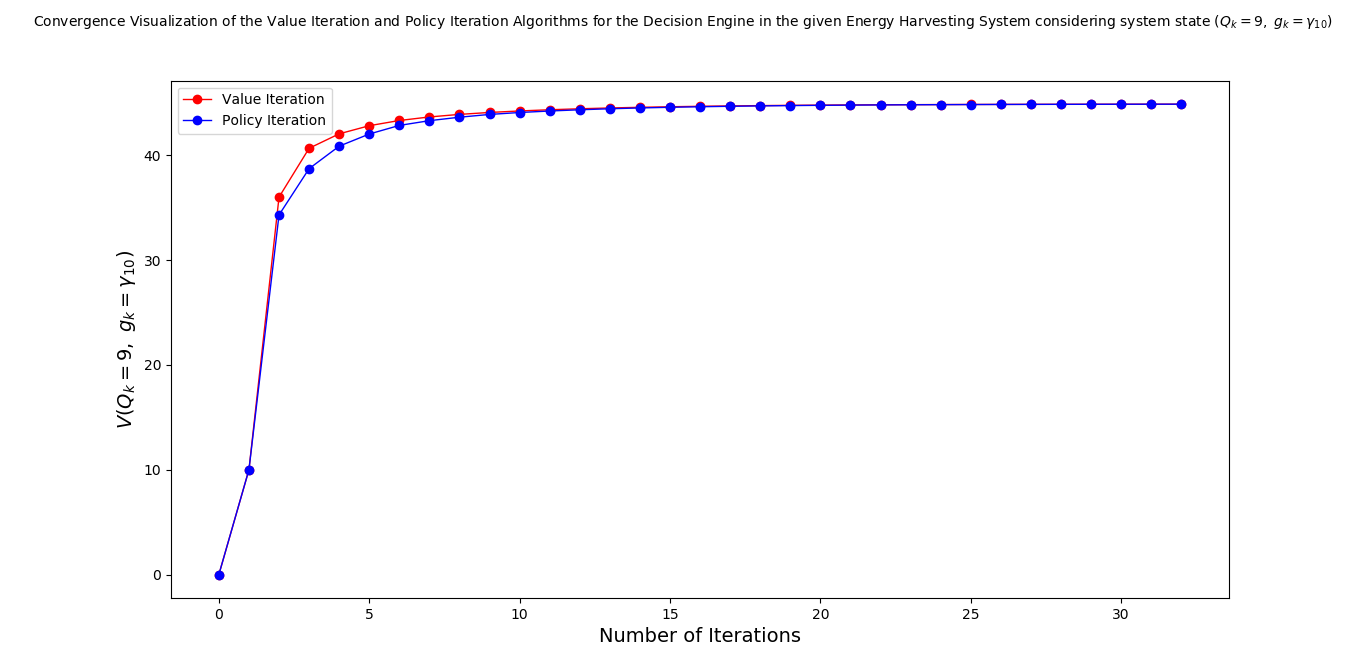
\includegraphics[width=1.0\textwidth]{Convergence_Analysis_Energy_Harvesting_Node_Better_Aesthetics.png}
\caption{Convergence Visualization of the Value Iteration and Policy Iteration Algorithms for the Decision Engine in the given Energy Harvesting System considering system state $(Q_k=9,\ g_k=\gamma_{10})$}
\label{fig:mesh1}
\centering
\end{figure}
\begin{figure}[t]
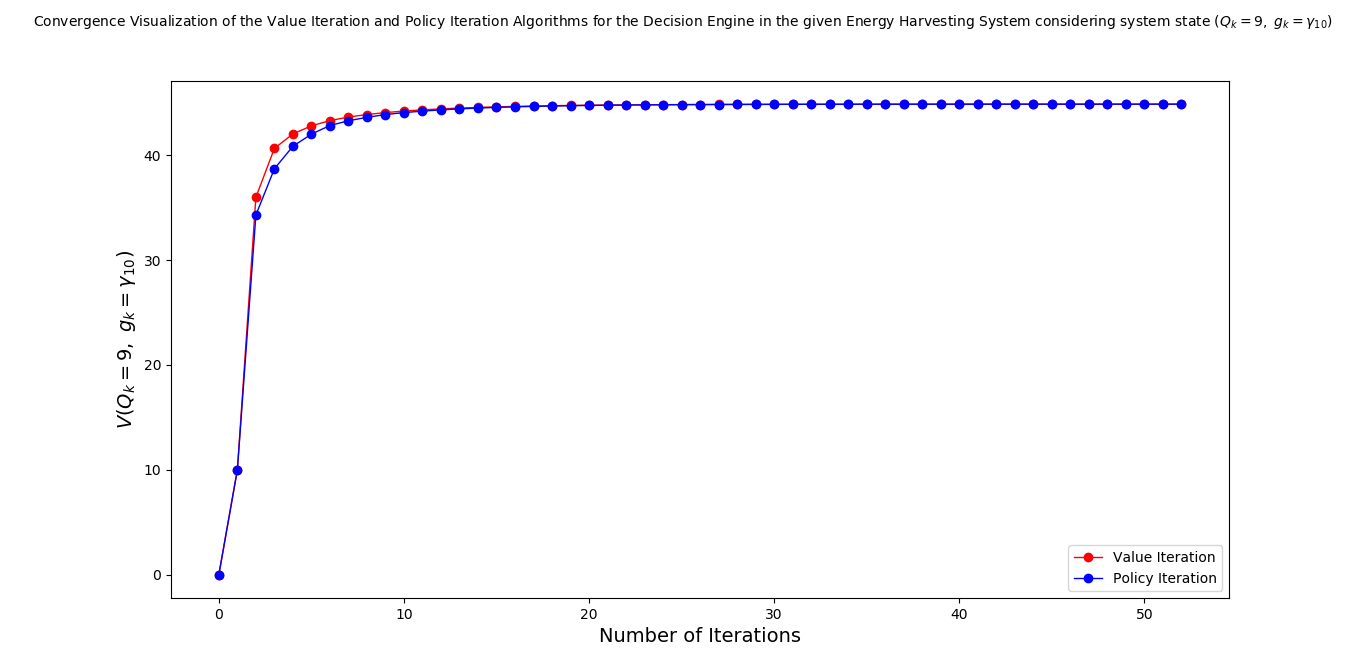
\includegraphics[width=1.0\textwidth]{Convergence_Analysis_Energy_Harvesting_Node_Increased_Confidence.png}
\caption{Convergence Visualization of the Value Iteration and Policy Iteration Algorithms for the Decision Engine in the given Energy Harvesting System considering system state $(Q_k=9,\ g_k=\gamma_{10})$ - Increased number of iterations to prove convergence}
\label{fig:mesh2}
\centering
\end{figure}
\begin{figure}[t]
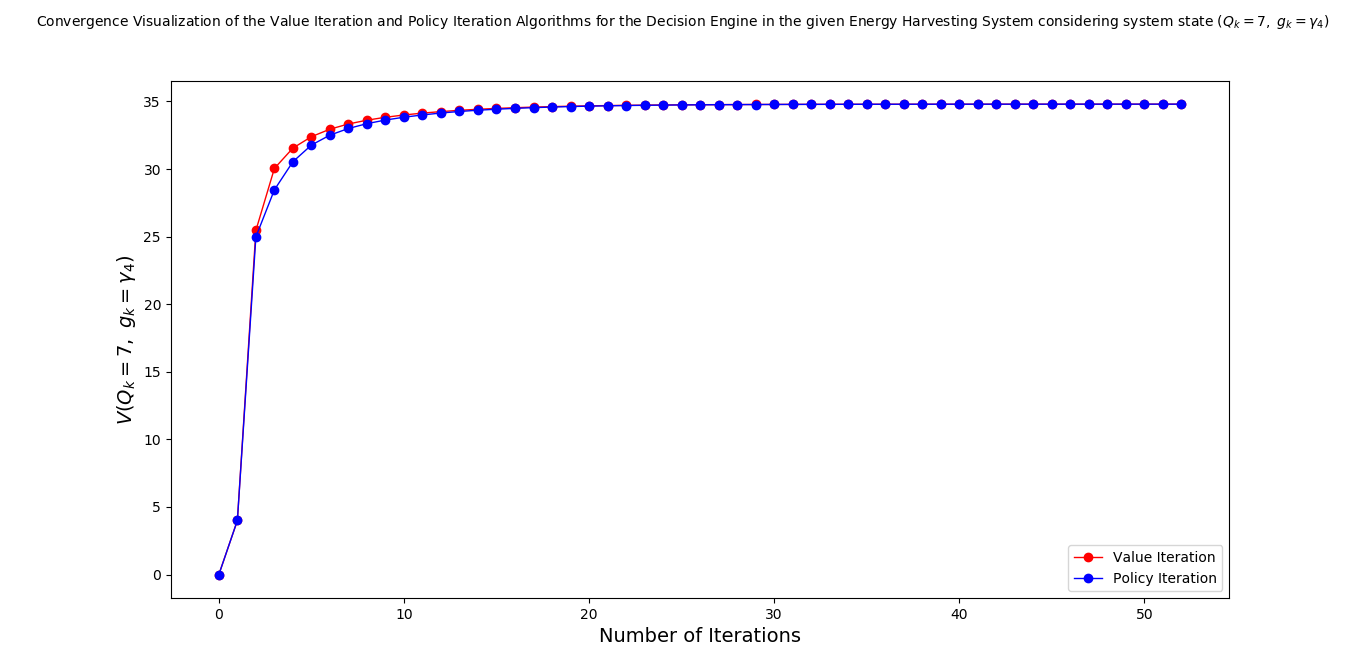
\includegraphics[width=1.0\textwidth]{Convergence_Analysis_Energy_Harvesting_Node_Increased_Confidence_7_4.png}
\caption{Convergence Visualization of the Value Iteration and Policy Iteration Algorithms for the Decision Engine in the given Energy Harvesting System considering system state $(Q_k=7,\ g_k=\gamma_{4})$}
\label{fig:mesh3}
\centering
\end{figure}
\begin{figure}[t]
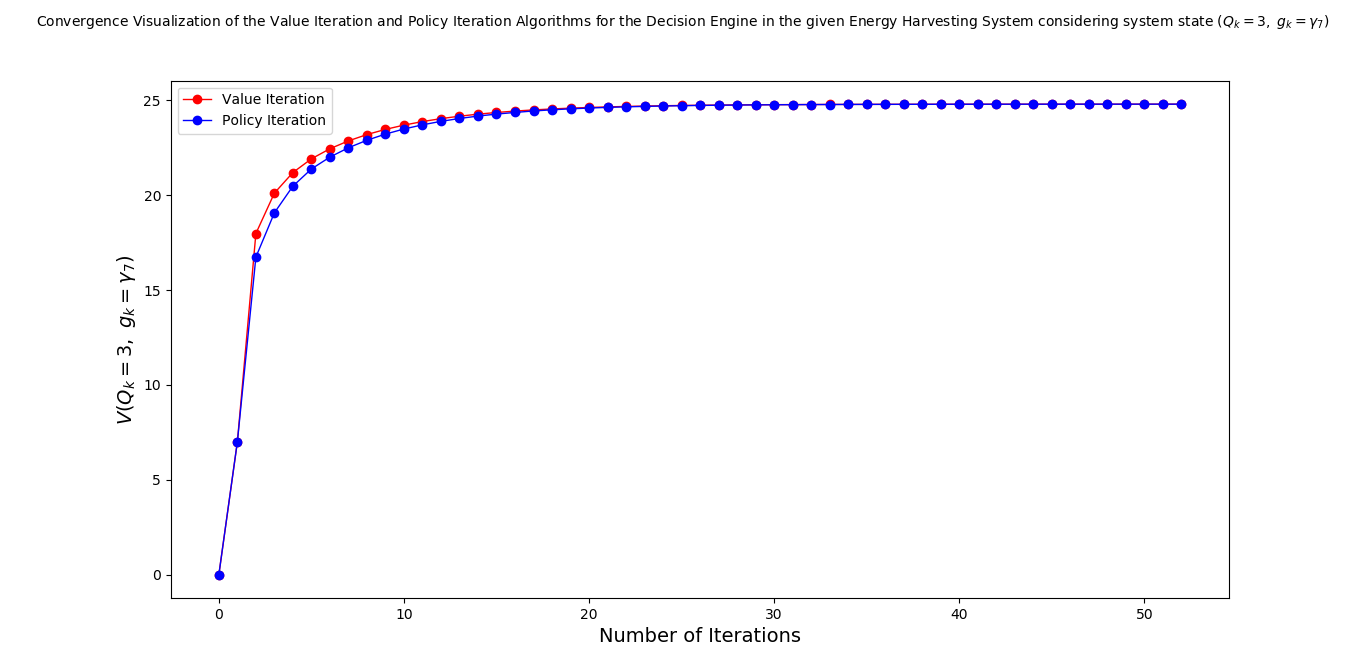
\includegraphics[width=1.0\textwidth]{Convergence_Analysis_Energy_Harvesting_Node_Increased_Confidence_3_7.png}
\caption{Convergence Visualization of the Value Iteration and Policy Iteration Algorithms for the Decision Engine in the given Energy Harvesting System considering system state $(Q_k=3,\ g_k=\gamma_{7})$}
\label{fig:mesh4}
\centering
\end{figure}
\begin{figure}[t]
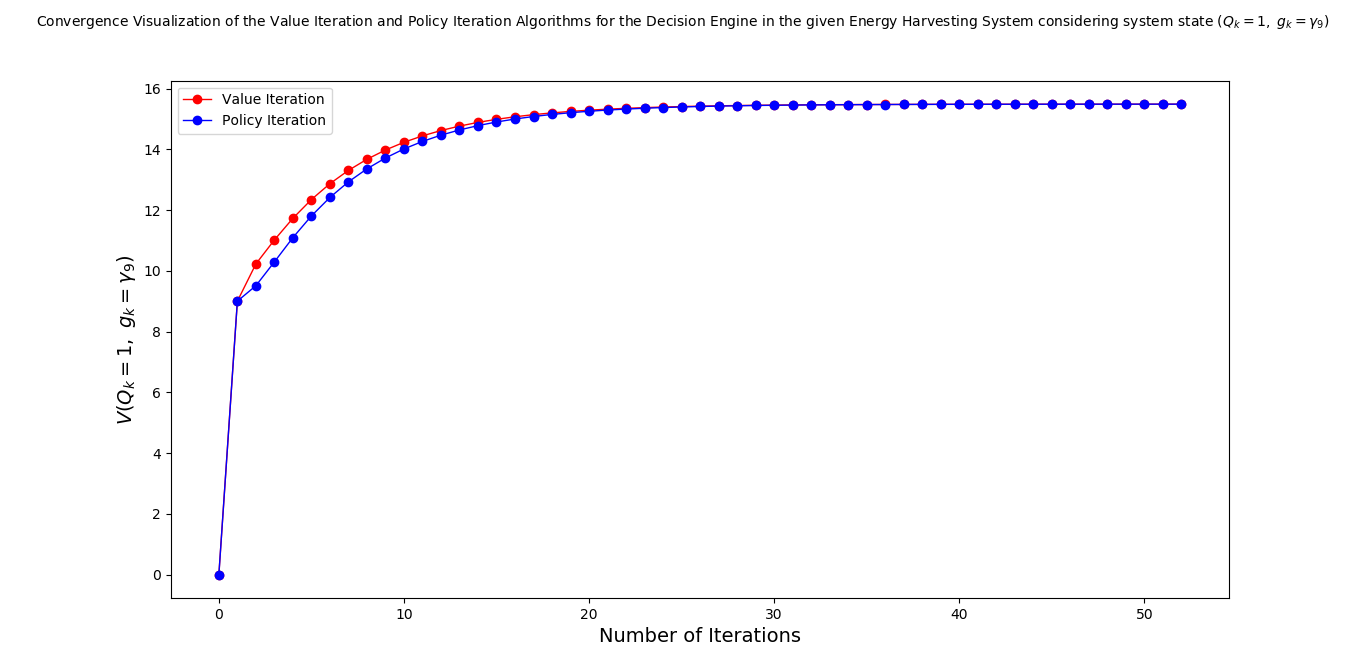
\includegraphics[width=1.0\textwidth]{Convergence_Analysis_Energy_Harvesting_Node_Increased_Confidence_1_9.png}
\caption{Convergence Visualization of the Value Iteration and Policy Iteration Algorithms for the Decision Engine in the given Energy Harvesting System considering system state $(Q_k=1,\ g_k=\gamma_{9})$}
\label{fig:mesh5}
\centering
\end{figure}
\begin{figure}[t]
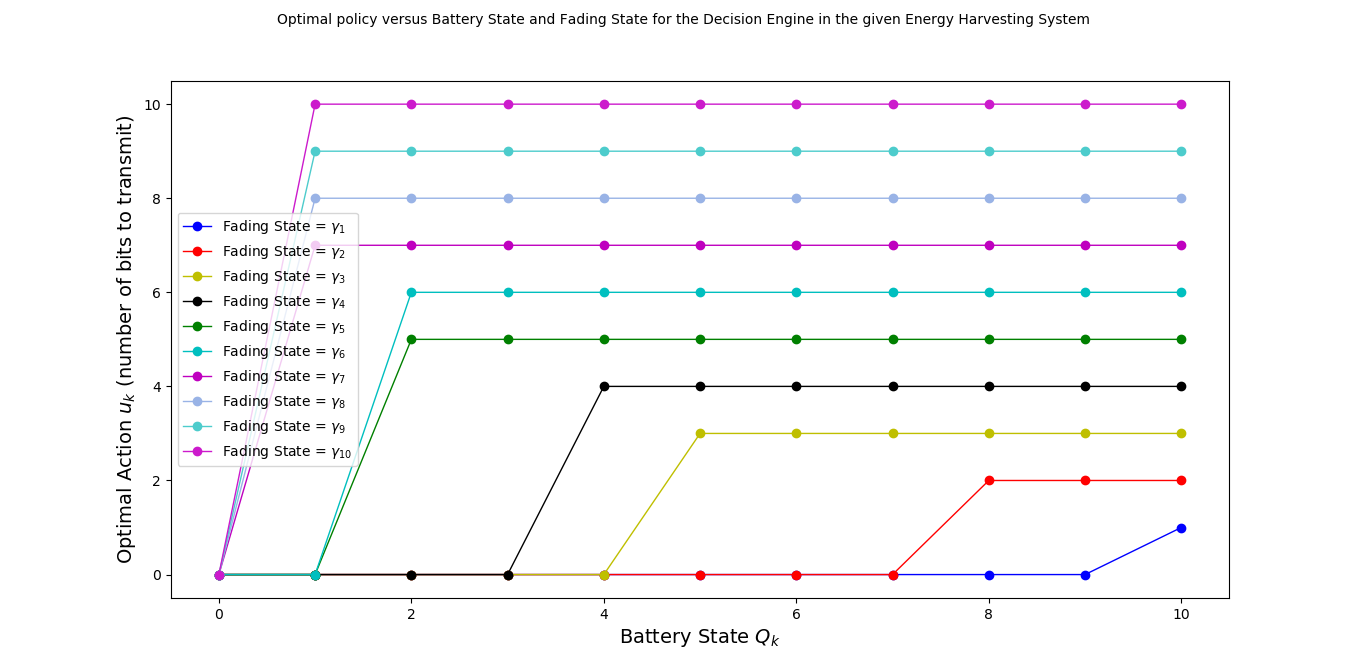
\includegraphics[width=1.0\textwidth]{Optimal_Policy_vs_Battery_State_with_Fading_State_Increased_Confidence.png}
\caption{Optimal policy versus Battery State and Fading State for the Decision Engine in the given Energy Harvesting System}
\label{fig:mesh6}
\centering
\end{figure}
\textit{Although Value Iteration and Policy Iteration are comparable in their performance due to smaller state and action spaces in this process, we can see from the plots that Value Iteration is slightly faster than Policy Iteration.}
\end{document}